%!TEX TS-program = pdflatexmk

% Copyright (c) 2018 - 2022, Martin Scheidt (ISC license)
% Permission to use, copy, modify, and/or distribute this file for any purpose with or without fee is hereby granted, provided that the above copyright notice and this permission notice appear in all copies.

\documentclass[border=2]{standalone}

\usepackage[dev]{tikz-trackschematic}

\begin{document}
  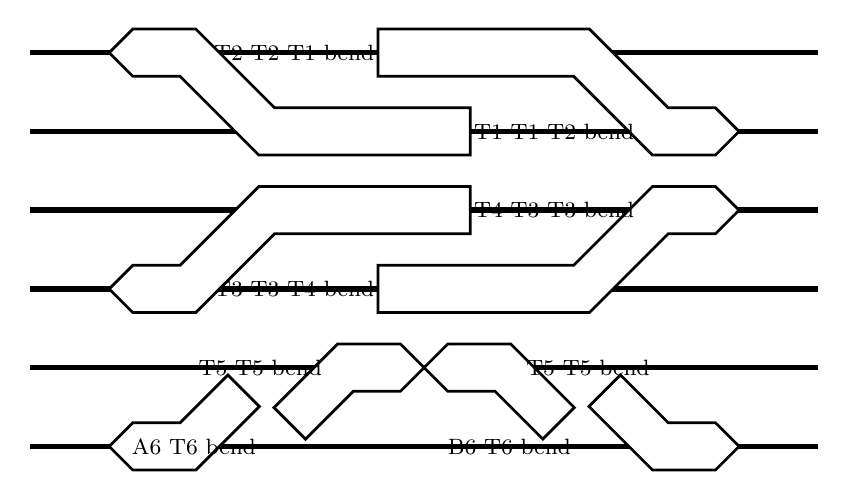
\begin{tikzpicture}
  
    \foreach \i in {1,2,...,6}{% base coordinate
      \coordinate (A\i) at ($(-1,0) + (0,-\i)$);
      \coordinate (B\i) at ($( 9,0) + (0,-\i)$);
    }

    \foreach \i in {1,2,...,6}{% draw main tracks on base coordinate
      \maintrack (A\i) --   (B\i);
    }

    \foreach \i in {1,2,...,6}{% coordinates for testing symbols
      \coordinate (T\i-0) at ($(0,0) + (0,-\i)$);
      \coordinate (T\i-1) at ($(1,0) + (0,-\i)$);
      \coordinate (T\i-2) at ($(2,0) + (0,-\i)$);
      \coordinate (T\i-3) at ($(3,0) + (0,-\i)$);
      \coordinate (T\i-4) at ($(4,0) + (0,-\i)$);
      \coordinate (T\i-5) at ($(5,0) + (0,-\i)$);
      \coordinate (T\i-6) at ($(6,0) + (0,-\i)$);
      \coordinate (T\i-7) at ($(7,0) + (0,-\i)$);
      \coordinate (T\i-8) at ($(8,0) + (0,-\i)$);
    }

    \train[forward, length=5cm,
      bend right at={(T1-6)}, bend left at={(T2-7)},
      shift label={(T1-6)}, label align=left] at (T2-8) label (T2 T2 T1 bend);
    \train[forward, length=5cm,
      bend left at={(T4-6)},bend right at={(T3-7)},
      shift label={(T4-6)}, label align=left] at (T3-8) label (T3 T3 T4 bend);
    \train[backward, length=5cm,
      bend right at={(T1-1)}, bend left at={(T2-2)},
      shift label={(T2-2)}, label align=right] at (T1-0) label (T1 T1 T2 bend);
    \train[backward, length=5cm,
      bend left at={(T4-1)},bend right at={(T3-2)},
      shift label={(T3-2)}, label align=right] at (T4-0) label (T4 T3 T3 bend);
    \train[backward, length=2cm,
      bend left at={(T6-1)},
      shift label={(T6-1)}, label align=left] at (T6-0) label (A6 T6 bend);
    \train[forward, length=2cm,
      bend right at={(T5-3)},
      shift label={(T5-2)}, label align=right] at (T5-4) label (T5 T5 bend);
    \train[backward, length=2cm,
      bend right at={(T5-5)},
      shift label={(T5-6)}, label align=left] at (T5-4) label (T5 T5 bend);
    \train[forward, length=2cm,
      bend left at={(T6-7)},
      shift label={(T6-7)}, label align=left] at (T6-8) label (B6 T6 bend);

  \end{tikzpicture}
\end{document}